% Can Zhou, 2020
% Star the repo if it helps you!
% Repo link: https://github.com/Can-ZHOU/Nottingham-FYP-Template

\documentclass[12pt, a4paper, twoside]{extarticle}
% Changing margins if you need :p
\usepackage[left=2.5cm,right=2.5cm,top=2cm,bottom=2cm]{geometry}
\usepackage[T1]{fontenc}
\usepackage[utf8]{inputenc}
\usepackage{cite}
\usepackage{float}
\usepackage{graphicx}
\usepackage{enumerate}

%------------------------Style, changing it if you need :)-----------------------
% If you have a long project title, 
% maybe you need to adjust the values after \vskip.
\makeatletter

% Set font. Default: Times
% \rmdefault -> Times
% \sfdefault -> Courier 
% \ttdefault -> Helvetica
\renewcommand{\familydefault}{\rmdefault}

\def\email#1{\gdef\@email{#1}}
\def\studentid#1{\gdef\@studentid{#1}}
\def\supervisor#1{\gdef\@supervisor{#1}}

\def\maketitle{
	\thispagestyle{empty}
	\vfill
	\begin{center}
		\centering{
		
\includegraphics[width=0.5\columnwidth]{images/nottingham-logo.png}} \par
		\vskip 1.8in \par
		\LARGE {\bf Project Proposal:} \par
		\vskip 5mm
		\LARGE {\bf \@title}
		\vskip 1.2in   
		\Large {\bf \@author} \par
		\vskip 5mm
		\Large {\bf \@studentid} \par
		\vskip 5mm
		\Large {\bf \@email} \par
		\vskip 10mm
		\Large {\bf Supervised by \@supervisor}
		\vskip 1.8in
		\Large {School of Computer Science, University of Nottingham}
	\end{center}
	\vfill
	\clearpage
}

\def\body{
\pagenumbering{arabic}
% Delete the indent
\setlength{\parindent}{0pt}
}
\makeatother

%--------------------------Change this part!------------------------------------
\title{Your Project Title}
\author{Yor Name}
\studentid{Student ID}
\email{Your Email}
\supervisor{Your Supervisor}

\begin{document}

\maketitle

\body

% Background and Motivation-----------------------------------------------------
\section{Background and Motivation}

\subsection{Using subsection}
Your project's background and motivation. \\
Example citation \cite{bradley1978robustness}.

% Aim and Objective-------------------------------------------------------------
\section{Aim and Objective}
Your aim and Objective. \\ \\
List examples:
\begin{itemize}
	\item This is the first item
	\item This is the second item
\end{itemize}
\begin{enumerate}
	\item The first item
	\item The second item
\end{enumerate}

% Project Plan -----------------------------------------------------------------
\section{Project Plan}
Your project plan. \\ \\
Custom list example:
\begin{enumerate}[A]
	\item The first item
	\item The second item
\end{enumerate}
% Gnatt chart. Modifying the image in images folder.
\begin{figure}[htbp] 
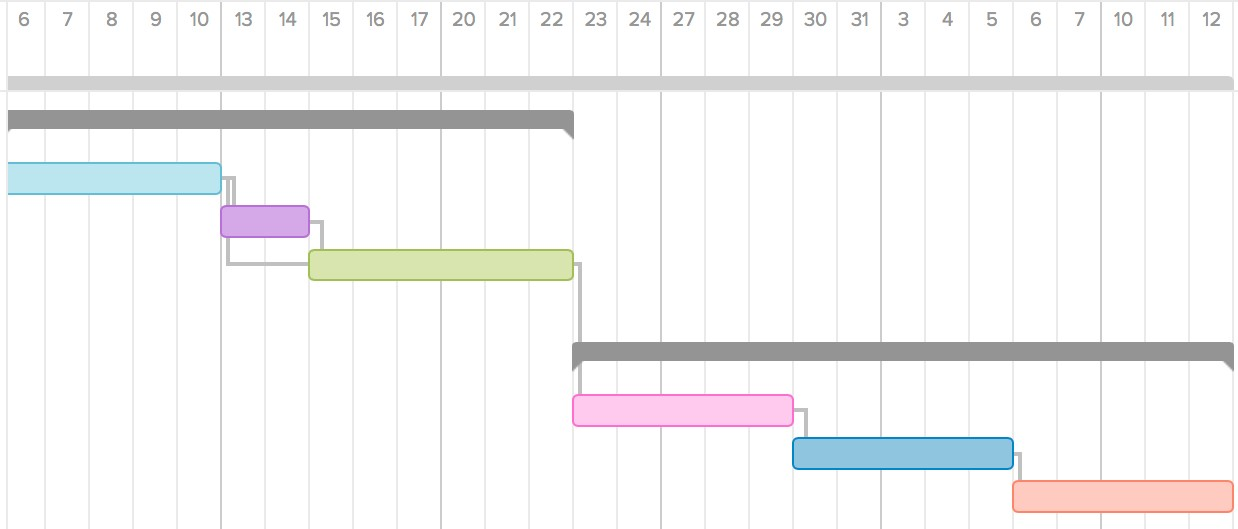
\includegraphics[width=1\columnwidth]{images/Gantt_Chart.jpg}
\caption{Gantt Chart}
\label{fig:1} 
\end{figure}

\newpage
\bibliographystyle{plain}
\bibliography{bibliography}

\end{document}
